\chapter{Inside Sin}
\begin{enumerate}
	\item \formation{\tidus}{\kimahri}{\auron}
	\item Walk along the path, flee from all encounters.
	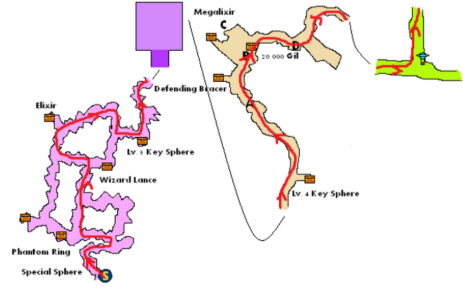
\includegraphics{graphics/sinpath}
	\item Before Seymour Omnis, \formation{\tidus}{\yuna}{\auron}
	\item Go up the steps, \sd
\end{enumerate}
\begin{battle}[80000]{Seymour Osmosis}
\begin{itemize}
	\yunaf Defend
	\tidusf Armor Break
	\item \textit{If Armor Break Hit:}
	\begin{itemize}
		\auronf Defend
		\summon{\bahamut}
		\bahamutf Attack
	\end{itemize}
	\item \textit{If Armor Break Missed:}
	\begin{itemize}
		\switch{\auronf}{\rikku}
		\rikkuf \od\ Mix Spherimorph Throwable + HiPot/MegaPot/XPot/Mega Phoenix
		\yunaf Cure Mortiphasm
		\tidusf Armor Break
		\summon{\bahamut}
		\bahamutf Attack
	\end{itemize}
\end{itemize}
\end{battle}
\begin{enumerate}
	\item \sd, walk north.
	\item \formation{\tidus}{\kimahri}{\auron}
	\item Make sure that \rikku's \od\ is charged
	\item Turn left onto the bridge, go onto the next screen. \save if needed.
	\item Complete the minigame, picking up the eggs and avoiding the crystals.
\end{enumerate}
\begin{spheregrid}
\begin{itemize}
	\item \textit{Bahamut Ending:}
	\begin{itemize}
		\item \textit{If you got 2/4 \textbf{Return Spheres}:}
		\begin{itemize}
			\yunaf Attribute Sphere \rikku's +3 Agi (hold L)
			\item Return Sphere ($\downarrow \downarrow \leftarrow \leftarrow$) or Friend Sphere ($\downarrow \leftarrow$) there
			\item Go down, picking up Agi+4, Spare Change, Agi+4
		\end{itemize}
		\item \textit{If you got 0 \textbf{Return Spheres}:}
		\begin{itemize}
			\yunaf Attribute Sphere \rikku's +3 Agi (hold L)
			\yunaf Go right, getting +4 Agi, +4 Agi
		\end{itemize}
		\tidusf If you didn't get a \textbf{Zombie Strike} weapon, then go back and learn Zombie Strike
		\rikkuf If no \od, use Skill Sphere to learn Armor Break
	\end{itemize}
	\item \textit{Quick Hit Ending:}
	\begin{itemize}
		\rikkuf Unlock Level 2 Key Sphere
		\item Move Up, Left
		\item Quick Hit
		\yunaf Use White Magic Sphere to learn Haste
		\yunaf Use Skill Sphere to learn Quick Hit
		\tidusf If you didn't get a \textbf{Zombie Strike} weapon, then go back and learn Zombie Strike
	\end{itemize}
\end{itemize}
\end{spheregrid}
\begin{enumerate}[resume]
	\item Walk up to Ject, \cs[4:30]
\end{enumerate}
\begin{battle}[180000]{Braska's Final Aeon}
\begin{itemize}
	\item \textit{Bahamut Ending:}
	\begin{itemize}
		\switch{\yuna}{\rikku}
		\rikkuf \od\ Mix Grenade + HP Sphere or Armor Break
		\tidusf Talk
		\switch{\auron}{\yuna}
		\summon{\bahamut}
		\bahamutf Attack
	\end{itemize}
	\item \textit{Quick Hit Ending:}
	\begin{itemize}
		\yunaf Haste \yuna
		\tidusf Talk
		\switch{\auron}{\rikku}
		\rikkuf \od\ Mix HP Sphere + Grenade for Chaos Grenade
		\yunaf Quick Hit
		\tidusf Talk
		\yunaf Quick Hits until out of MP
		\summon{\bahamut}
		\bahamutf Attack
	\end{itemize}
\end{itemize}
\end{battle}
\begin{enumerate}[resume]
	\item \cs+\skippablefmv[4:00]
\end{enumerate}
\begin{battle}{Possesed Aeons}
\begin{itemize}
	\item \textit{Bahamut Ending:}
	\begin{itemize}
		\item Spare Change as follows:
		\begin{itemize}
			\valeforf \num{20000} Gil
			\ifritf \num{30000} Gil
			\ixilonf \num{30000} Gil
			\bahamutf \num{40000} Gil
			\shivaf All Remaining Gil
		\end{itemize}
	\end{itemize}
	\item \textit{Quick Hit Ending:}
	\begin{itemize}
		\yunaf Elixer \yuna
		\item Option 1:
		\begin{itemize}
			\yunaf Quick Hit
			\yunaf Haste \yuna
			\yunaf Quick Hit
		\end{itemize}
		\item Option 2:
		\begin{itemize}
			\valeforf Waterga
			\ifritf Waterga
			\shivaf Waterga
			\bahamutf Waterga x2
			\ixilonf Switch Weapon to Mage's Staff
			\tidusf Defend
			\yunaf Waterga
		\end{itemize}
	\end{itemize}
\end{itemize}
\end{battle}
\begin{enumerate}[resume]
	\item \cs[1:40]
\end{enumerate}
\begin{battle}[99999]{Yu Yevon}
\begin{itemize}
	\item Anyone: Zombie Attack
	\item Anyone: Throw Phoenix Down
\end{itemize}
\end{battle}

	